% !TEX encoding = UTF-8
% !TEX TS-program = pdflatex
% !TEX root = ../tesi.tex

%**************************************************************
\chapter{Volume Rendering e Qt}
\label{cap:teoria-stage}
%**************************************************************

%**************************************************************
\section{Radiologia e rendering}
\intro{Concetti di base, teoria, algoritmi e gestione/caricamento immagini DICOM}\\

\subsection{Visualizzare informazioni}\label{sec:visualizzare-informazioni}
Visualizzare fa parte della nostra vita quotidiana: dalle mappe satellitari alla computer grafica dell'industria dell'intrattenimento, possiamo trovare esempi di visualizzazione praticamente ovunque. Ma che cosa significa visualizzare informazioni? Informalmente, visualizzare è la trasformazione di dati o informazioni in immagini. Visualizzare coinvolge la vista e la potenza di elaborazione della mente, con un risultato semplice ed efficace per comunicare informazioni complesse e/o voluminose.
\\
Tuttavia, forse la migliore definizione di visualizzazione si trova negli esempi. In molti casi la visualizzazione sta influenzando la vita delle persone e compiendo imprese che alcuni anni fa sarebbero state inimmaginabili, come nella medicina moderna, ambito su cui ci concentreremo.

\subsection{Volumi radiologici}\label{sec:volumi-radiologici}
Le tecniche di diagnostica per immagini, soprattutto in radiologia, sono diventate un importante strumento nella medicina moderna. Ci concentreremo su tecniche come la tomografia computerizzata (TC) e la risonanza magnetica (RM).
\\
Queste teniche utilizzano dei processi di acquisizione e campionamento per raccogliere informazioni sull'anatomia interna di un paziente. Queste informazioni sono raccolte in forma di piani di taglio o in immagini in sezione trasversale di un paziente, in maniera simile a come accade per radiografie a raggi X convenzionali. La TC utilizza un fascio di raggi X per acquisire i dati, mentre la RM utilizza un forte campo magnetico unito a  impulsi a radiofrequenza. Varie teniche matematiche vengono utilizzate per ricostruire i piani di taglio da salvare, dopodichè solitamente, questi vengono raccolte in un volume di dati.
\\
Un'immagine radiologica, o una fetta del volume nel nostro caso, è acquisita come una serie di valori che rappresenta l'attenuazione dei raggi X (nella TC) o il rillassamento dello spin di un atomo. Ogni immagine contiene tutti questi dati in un array, o in una matrice, tuttavia la quantità di dati è così grande che è impossibile comprenderli nella loro forma "grezza". Per questo, assegnandogli una scala di grigi e visualizzandoli su uno schermo, si riesce finalmente a visualizzare la struttura, permettendoci di visualizzare ciò che il computer vede come un insieme di valori come una sezione del corpo umano.

\subsection{Basi di rendering}\label{sec:basi-rendering}
La computer grafica è il processo di generare immagini utilizzando il computer, questo processo viene chiamato rendering. Ci sono molti tipi di rendering, dal disegno 2D a tecniche 3D sofisticate. In questa sezione vedremo le basi del rendering 3D.
\\
Nel mondo reale quando guardiamo un oggetto, per esempio una scatola, i raggi di luce emessi da una sorgente luminosa (per esempio il sole) sono emessi in tutte le direzioni. Alcuni di questi colpiscono la scatola che ne assorbe una parte di luce e ne riflette il resto. Una parte di questa luce riflessa potrebbe dirigersi verso di noi ed entrare nei nostri occhi, se questo succede noi riusciamo a vedere l'oggetto. Allo stesso modo se della luce colpisce il terreno una parte si rifletterà nei nostri occhi.

\begin{figure}[h]
    \centering
    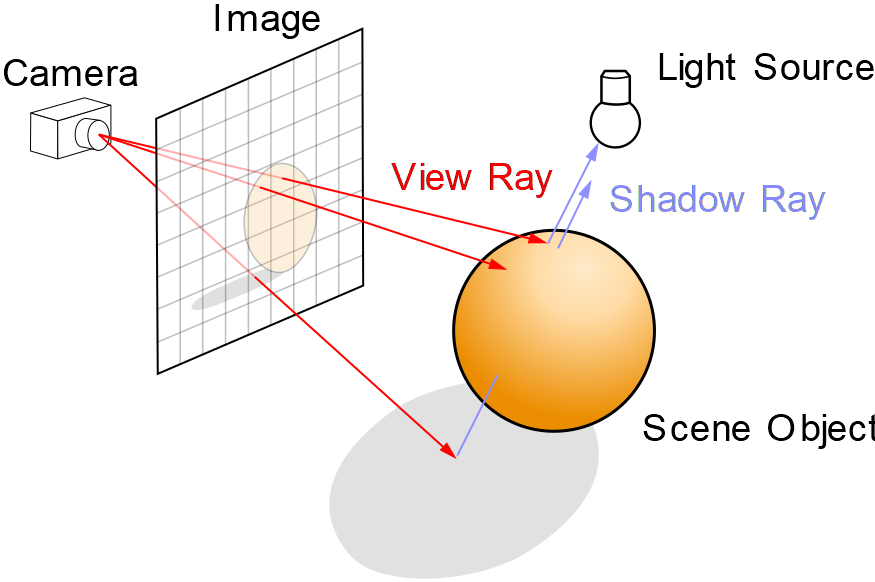
\includegraphics[width=0.5\textwidth]{immagini/volumerendering/ray_tracing_diagram.png}
    \caption{\textit{Algoritmo di Ray-Tracing}}
    \textbf{Fonte}: \href{https://en.wikipedia.org/wiki/Ray_tracing_(graphics)}{wikipedia.org/wiki/Ray\_tracing}
    \label{fig: Algoritmo di Ray-Tracing}
\end{figure}

Una tecnica comune ed efficace per la computer grafica 3D è il ray-tracing, a volte chiamata anche ray-casting. Il ray-tracing simula l'interazione della luce con gli oggetti, seguendo il percorso di ogni raggio. Di solito, si segue il raggio dall'indietro, dalla posizione dell'osservatore (la camera nello schema) nel mondo per determinare che cosa il raggio colpisce. La direzione del raggio quindi, è la direzione che si sta osservando. Quando un raggio colpisce un oggetto, possiamo determinare se quel punto è illuminato da una sorgente di luce: questo viene fatto tracciando un raggio dal punto di intersezione alla luce: se il raggio colpisce qualcos'altro prima di raggiungere la sorgente luminosa, allora quella luce non contribuirà a illuminare il punto. Se ci sono N sorgenti luminose, questo andrà fatto per oguna di esse.
\\
Per chi non avesse mai sentito parlare del ray-tracing, sarà sorprendente scoprire che non è quasi mai usato nella grafica real-time. Questo perchè il ray-tracing è un processo molto lento e dispendioso in termini di risorse, oltre al fatto che fino a pochi anni fa era possibile implementarlo solo via software, per questo sono state sviluppate altre teniche che generano immagini sfruttando meglio l'accellerazione hardware.
\\
La spiegazione fino a questo punto ha assunto che stessimo facendo il render di un oggetto solido. Tuttavia, oggetti come nuvole, l'acqua, la nebbia sono "traslucidi" o diffondono la luce che li attraversa, questi oggetti non possono essere renderizzati utilizzando esclusivamente le interazioni sulle superfici. Dobbiamo invece considerare le proprietà mutevoli all'interno dell'oggetto per mostrarlo correttamente. Ci riferiamo quindi a due modelli di rendering:
\begin{itemize}
\item surface rendering: esegue il render della superficie di un oggetto;
\item volume rendering: esegue il rendering della superficie e dell'interno di un oggetto.
\end{itemize}

Le tecniche di volume rendering ci consentono di vedere la "disomogeneità" all'interno degli oggetti. Nella TC per esempio, possiamo riprodurre realisticamente immagini a raggi X considerando i valori di intensità sia sulla superficie che all'interno. Vedremo più dettagli sul volume rendering nella prossima sezione, ma tornando all'esempio del ray-tracing, si può immaginare come i raggi non interagiscano solo con la superficie di unh oggetto, ma anche con ciò che è al suo interno.

%**************************************************************
\section{Volume rendering}
\subsection{Basi di volume rendering}\label{sec:volume-rendering-details}
Finora ci siamo concentrati sulla visualizzazione di dati tramite l'utilizzo di primitive come punti, linee e poligoni. Per molte applicazioni questo è chiaramente il metodo migliore per rappresentarli, tuttavia alcune applicazioni ci richiedono di visualizzare dati che sono "volumetrici", più comunemente chiamati immagini 3D o set volume di dati (volume datasets). Per esempio, nell'imaging biomedico potremmo aver bisogno di visualizzare dati ottenuti da una RM, una TC, un microscopio o un'ecografia. Anche l'analisi meteorologica e altre simulazioni producono grandi quantità di dati volumetrici in tre o più dimensioni che richiedono tecniche di visualizzazione efficaci.
\\
Vedremo ora più in dettaglio alcuni metodi di volume rendering che usano...?
\\
Considerando che il rendering volumetrico è tipicamente usato per generare immagini che rappresentano un intero set 3D in un'immagine 2D, bisogna prestare attenzione ad alcuni punti: una classificazione deve essere eseguita per assegnare colore e opacità alle regioni all'interno del volume, e devono essere definite delle tecniche di illuminazione volumetrica per migliorare il risultato.

\subsection{Volume rendering Image-Order}\label{sec:volume-image-order}
Il volume rendering Image-Order è spesso chiamato "ray casting" o "ray tracing". L'idea di base è determinare il valore di ogni pixel dell'immagine, inviando un raggio dalla posizione del pixel nella scena, secondo i valori della visuale corrente. A quel punto si  valutano i dati incontrati lungo il raggio, per calcolare il valore del pixel. Come vedremo, il ray casting è una tecnica che può essere ustata per fare il render di qualsiasi dataset 3D producendop una grande varietà di immagini, ed è relativamente semplice estenderlo in modo da utilizzarlo per un set di dati volumetrici per lavorare su "griglie" ben strutturate. Sfortunatamente, il ray casting è un processo abbastanza lento, pertanto si utilizzano una serie di metodi di accelerazione per migliorare le prestazioni, sacrificando alcuna memoria aggiuntiva o parte di flessibilità dell'algoritmo.

\begin{figure}[h]
    \centering
    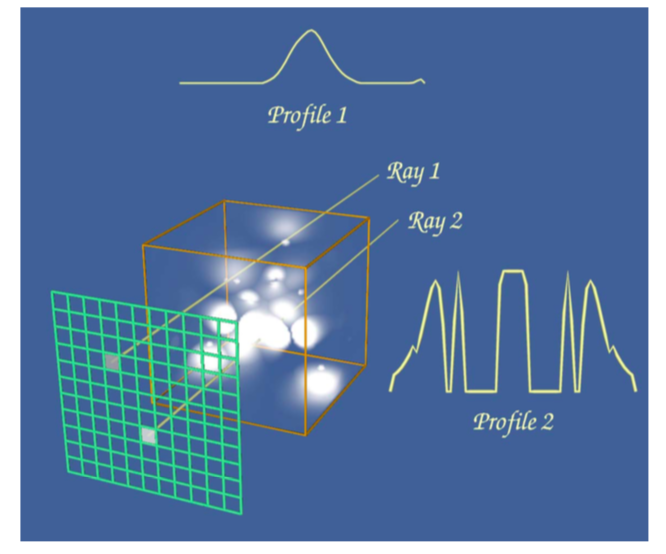
\includegraphics[width=0.5\textwidth]{immagini/volumerendering/imageorder.png}
    \caption{\textit{Volume Rendering Image-Order}}
    \textbf{Fonte}: \href{https://lorensen.github.io/VTKExamples/site/VTKBook/07Chapter7/}{VTKBook/Chapter7/}
    \label{fig: Volume Rendering Image-Order}
\end{figure}

Un esempio del processo di ray casting è illustrato nell'immagine qui sopra. Questo esempio utilizza una proiezione ortografica della camera standard, di conseguenza tutti i raggi sono paralleli l'un l'altro e perpendicolari alla vista (anche chiamata "view plane"). I dati processati lungo ciascun raggio sono processatti con una funzione specifica, che in questo caso determina il valore massimo incontrato e lo converte ad una scala di grigi, dove il valore minimo è mappato come nero trasparente, e il massimo valore è mappato come bianco opaco.

\subsection{Volume rendering Object-Order}\label{sec:volume-object-order}
Il volume rendering Object-Order processa i valori nel volume basandosi sull'organizzazione dei voxel nel dataset e sulle impostazioni della visuale corrente. Quando un metodo "alpha compositing" è utilizzato, i voxel vanno processati in ordine "front-to-back" o "back-to-front" per ottenere risultati corretti. Se si sfrutta l'hardware dedicato, è preferibile utilizzare l'ordine "back-to-front" in quanto si evita di calcolare dei valori extra riguardo la trasparenza. Al contrario, se si utilizza il render software, l'ordine "front-to-back" è più comune in quanto è possibile evitare di processare ulteriori dati quando un pixel raggiunge la "piena opacità". Alcune tecniche, come la MIP, possono essere processate in qualsiasi ordine per ottenere risultati corretti.

\begin{figure}[h]
    \centering
    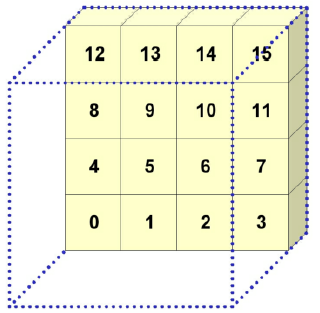
\includegraphics[width=0.5\textwidth]{immagini/volumerendering/objectorder.png}
    \caption{\textit{Volume Rendering Object-Order}}
    \textbf{Fonte}: \href{https://lorensen.github.io/VTKExamples/site/VTKBook/07Chapter7/}{VTKBook/Chapter7/}
    \label{fig: Volume Rendering Object-Order}
\end{figure}

La figura qui sopra rappresenta un approccio "back-to-front" per calcolare i voxel: si parte dal voxel più lontano rispetto alla visuale, e si prosegue visitandoli in ordine di distanza finchè non sono stati tutti visitati.

\subsection{Funzione di trasferimento}\label{sec:funzione-trasferimento}
Una funzione di trasferimento è responsabile della mappatura delle informazioni dei voxel in valori differenti come materiale, colore o trasparenza. Uno dei punti di forza del volume rendering, è che può gestire funzioni di trasferimento di complessità molto maggiore di una funzione "a passo binario". Questo è spesso necessario considerando che i dataset contengono più materiali e un metodo di classificazione non può sempre riuscire ad assegnare un singolo materiale ad un campione.

\begin{figure}[h]
    \centering
    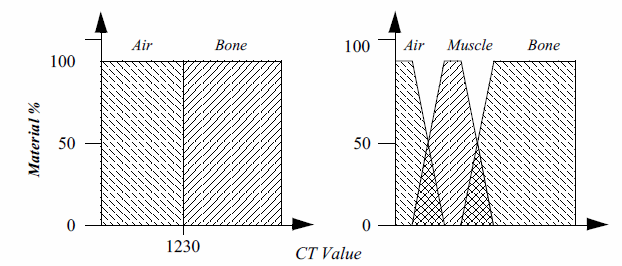
\includegraphics[width=0.5\textwidth]{immagini/volumerendering/functions.png}
    \caption{\textit{Semplice classificazione binaria (sinistra) e una transizione graduale tra aria a muscoli a ossa (destra).}}
    \textbf{Fonte}: \href{https://lorensen.github.io/VTKExamples/site/VTKBook/07Chapter7/}{VTKBook/Chapter7/}
    \label{fig: Volume Rendering Object-Order}
\end{figure}

Prendendo come esempio una TC, ora possiamo specificare una funzione di trasferimento che definisca una transizione graduale da aria, a muscoli, ad ossa, come mostrato nell'immagine qui sopra.

Altro???

\subsection{Regioni di interesse}\label{sec:regioni-di-interesse}
Un problema nel visualizzare dati volumetrici, è che se volessi studiare alcuni dati al centro del volume, dovrei guardare a tutto ciò che c'è attorno nel dataset. Per esempio, se visualizzassi il dataset di un pomodoro, non riuscirei a vedere i semi perchè con tecniche come la MIP, vedrei tutta la polpa circostante.

\begin{figure}[h]
    \centering
    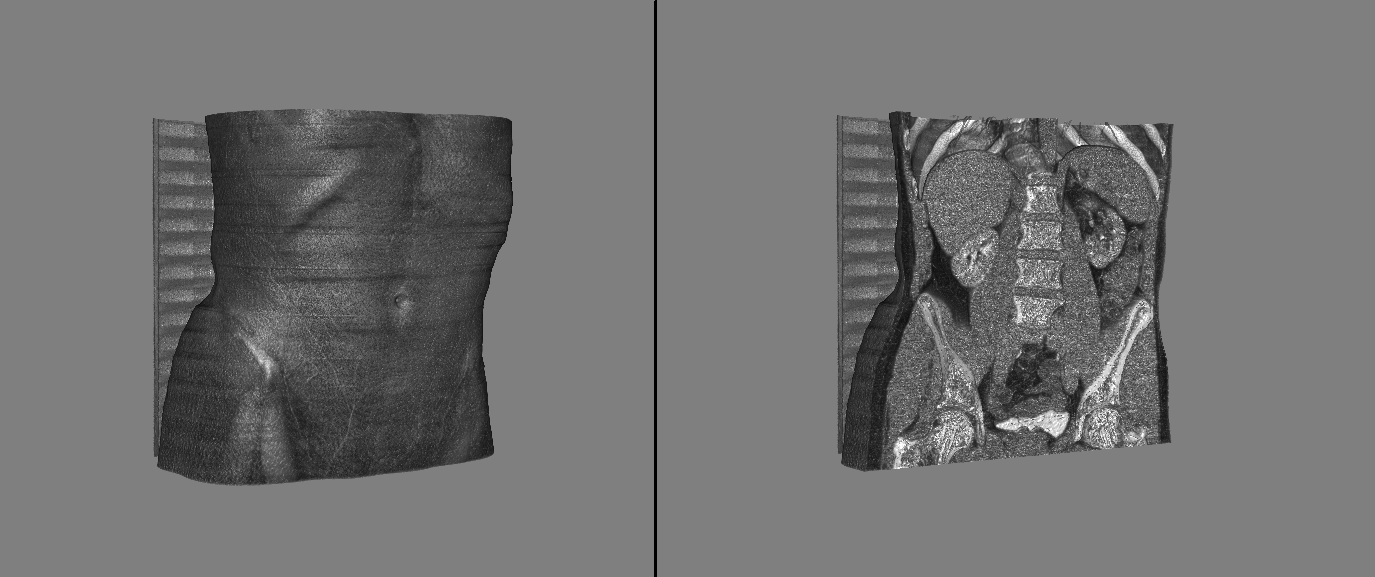
\includegraphics[scale=0.3]{immagini/volumerendering/regionofinterest.png}
    \caption{\textit{Esempio di volume rendering con regione di interesse, tagliando il volume.}}
    \textbf{Fonte}: Stage
    \label{fig: Volume Rendering Object-Order}
\end{figure}

Possiamo risolvere questo problema di visualizzazione interna, definendo una regione di interesse del nostro folume, e facendo il render quindi solo di una porzione del dataset come mostrato nella figura qui sopra. Ci sono molte tecniche per definire una regione di interesse: si potrebbe utilizzare i piani "far" e "near" della camera per escludere parti del volume; altrimenti si possono definire sei piani (un cubo quindi) per definire un sotto-volume da visualizzare, escludendo il resto all'esterno del cubo; si possono anche utilizzare più piani distinti per escludere sezioni in varie posizioni e orientamenti.

%**************************************************************
\section{VTK}
\intro{Funzionalità libreria, rendering, taglio, CPU/GPU e funzioni di trasferimento}\\
\subsection{Scelta della libreria}\label{sec:scelta-liberia}

\subsection{Oggetti di rendering}\label{sec:oggetti-rendering}

\subsection{Altro}\label{sec:aaa}

\subsection{Widget e interazione utente}\label{sec:widget-interazione}

%**************************************************************
\section{Integrazione con Qt}

%**************************************************************
\section{Software correlati}
\intro{Probabile menzione a Slicer3D, il principale software preso come riferimento}\\

%**************************************************************
\section{Strumenti CTK}

%**************************************************************
\section{Basi di ITK}

